\documentclass{article}
\usepackage[polish]{babel}
\usepackage[utf8]{inputenc}
\usepackage[T1]{fontenc}
\usepackage{graphicx}
\usepackage{enumitem}

\usepackage{fancyhdr}
\usepackage{lastpage}

\pagestyle{fancy}
\fancyhf{}

\rfoot{Strona \thepage \hspace{1pt} z \pageref{LastPage}}


\title{Specyfikacja implementacyjna projektu zespołowego "Symulator przewożenia pacjentów do szpitali w Polsce"}
\author{Michał Wójcik, Marek Nowakowski, Filip Olejniczak}
\date{18 listopada 2020}

\begin{document}

\maketitle

\tableofcontents
\pagebreak

\section{Informacje ogólne}
    "Symulator przewożenia pacjentów do szpitali w Polsce" to program, którego celem działania jest \textbf{symulacja} symulowanie \textbf{transportu pacjentów do szpitali} przy pomocy karetek pogotowia. Program jest uruchamiany bez podawania argumentów wejściowych. Po uruchomieniu programu użytkownikowi na środku ekranu pojawi się okienko programu wraz z interfejsem umożliwiającym dodanie użytkownikowi parametrów wejściowych w postaci pliku z pacjentami oraz pliku z szpitalami, drogrami i obiektami. Językiem programowania, w którym napisane będzie program jest Java 14, natomiast środowiskiem programistycznym IntelliJ IDEA.

\section{Diagram klas}

    \begin{center}
        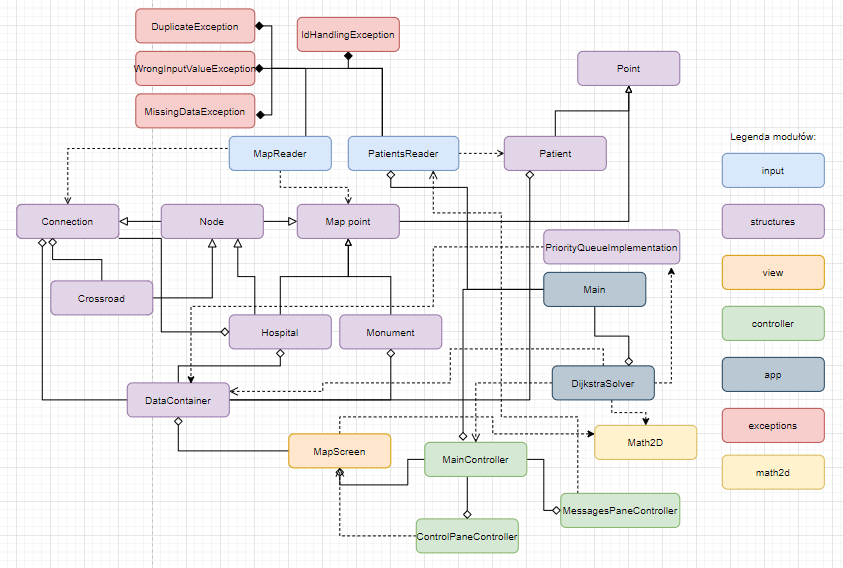
\includegraphics[scale=0.45]{diagramKlas.png}
    \end{center}

\section{Opis modułów/pakietów}
    \subsection{math2d}
    Pakiet math2d będzie zawierał klasy odpowiadające za przekształcenia matematyczne w kartezjańskim układzie współrzędnych. Klasy te będą wykorzystywane przez klasę z pakietu view do budowy mapy symulacji na podstawie danych zawartych w strukturach zdefiniowanych przez pakiet structures.

    \subsection{structures}
    Pakiet structures będzie zawierał klasy służące do reprezentacji oraz przechowywania danych w programie. Dane te będą dostarczne przez klasy zawarte w module input oraz klasy zawarte w module controller. Będzie również służył do reprezentacji elementów grafu, który w połączeniu z algorytmem zawartym w module app będzie służył do wyliczenia najkrótszej drogi między wszystkimi szpitalami.

    \subsection{input}
    Pakiet input będzie zawierał klasy odpowiedzialne za czytanie oraz obsługę danych z plików wejściowych. Podczas czytania tworzone będą instancje poszczególnych klas z pakietu structures, w których te dane będą przechowywane. Aby użytkownik programu mógł wykorzystać funkcjonalności udostępnione przez tą klasę, pakiet ten będzie powiązany z pakietem controller.

    \subsection{exception}
    W tym module znajdą się wyjątki, które zostaną użyte w konkretnych sytuacjach na etapie pobierania danych z pliku wejściowego, dlatego moduł będzie powiązany z modułem input, który odpowiada m.in za obsługę danych wejściowych. Moduł będzie również powiązany z modułem app w celu obsługi tych wyjątków.

    \subsection{controller}
    Moduł controller będzie zawierał klasy odpowiadające za obsługę interfejsu graficznego użytkownika. Pakiet ten będzie powiązany z wszystkimi pozostałymi pakietami w celu wywoływania odpowiednich metod (na obiektach z pakietu structures) z poziomu interfejsu użytkownika oraz wyświetleniu użytkownikowi ewentualnych błędów.

    \subsection{view}
    Moduł view będzie zawierał klasę odpowiadające za graficzną wizualizację symulacji w czasie rzeczywistym. Pakiet będzie zawarty w module controller, w którym to module klasy tego pakietu będą obsługiwane.

    \subsection{app}
    Pakiet będzie posiadał w sobie klasy sterujące działaniem programu oraz algorytmem znajdującym najkrótszą drogę do wszystkich szpitali. Pakiet znajdzie zastosowanie w pakiecie controller, gdzie będzie wykonywać niezbędne operacje w celu przeprowadzenia symulacji.



\section{Opis klas}
    \subsection{Math2D}
    Klasa zawarta w pakiecie math2d. Będzie ona posiadać metody, które umożliwią rozwiązywanie określonych zagadnień matematycznych z zakresu geometrii analitycznej, które są niezbędne do zbudowania modelu mapy:
    \begin{itemize}
        \item static Point calculateCrossing(Point p1, Point p2, Point l1, Point l2); \\
        metoda licząca punkt przecięcia się dwóch prostych, zdefiniowanych przez pary punktów.

        \item static double angleBetweenLines(Point p1, Point p2, Point l1, Point l2); \\
        metoda licząca miarę kąta pomiędzy dwiema prostymi, zdefiniowanymi przez pary punktów.

        \item static arePointsOnSameLine(Point p1, Point p2, Point p3); \\
        matoda ustalająca, czy wszystkie trzy punkty leżą na jednej prostej, czy nie,

    \end{itemize}
    Konstruktor klasy będzie bezargumentowy. Nie będzie ona również posiadać pól.

    \subsection{MapReader}
    Klasa zawarta w pakiecie input. Jej zadaniem jest odczytanie pliku (na podstawie instancji klasy BufferedReader, przekazanej jako argument konstruktora).
    Klasa będzie zawierać pola:
    \begin{itemize}
        \item BufferedReader reader;
        \item Set<Hospital> hospitals;
        \item Set<Monument> monuments;
        \item Set<Connection> connections;
    \end{itemize}
    Wszystkie pola będą inicjalizowane w konstruktorze.
    Klasa będzie zawierać metody:
    \begin{itemize}
        \item Set<MapPoint> readMapPoints(); \\
        zwracającą zbiór instancji klasy MapPoint (klas Hospital lub Monument),

        \item Set<Connection> readConnections(); \\
        zwracającą zbiór połączeń między szpitalami,

        \item MapPoint readMapPointInLine(String line); \\
        zwracającą obiekt MapPoint wczytany z zadanej linii,

        \item Connection readConnection(String line); \\
        zwracającą obiekt Connection wczytany z zadanej linii;
    \end{itemize}

    \subsection{PatientsReader}
    Klasa zawarta w pakiecie input. Jej zadaniem jest odczytanie pliku (na podstawie instancji klasy BufferedReader, przekazanej jako argument konstruktora).
    Klasa będzie zawierać pola:
    \begin{itemize}
        \item BufferedReader reader;
        \item List<Patient> patients;
    \end{itemize}
    Wszystkie pola będą inicjalizowane w konstruktorze.
    Klasa będzie zawierać metody:
    \begin{itemize}
        \item List<Patient> readPatients; \\
        zwracającą zbiór instancji klasy Patient,

        \item Patient readPatient(String line); \\
        zwracającą obiekt Patient wczytany z zadanej linii;
    \end{itemize}

    \subsection{PriorityQueueIplementation}
    Klasa zawierająca się w pakiecie structures. Będzie ona implementacją kolejki priorytetowej w postaci kopca. Klasa będzie posiadać pola:
    \begin{itemize}
        \item List<T> elements;
    \end{itemize}
    Metody:
    \begin{itemize}
        \item void put(T elem);
        \item  T pop();
        \item void heapUp(int lastId);
        \item void heapDown();
        \item boolean isRightChildBigger(int n, int leftChildId);
        \item boolean isChildBiggerThanParent(int parentId, int childId);
    \end{itemize}
    Konstruktor klasy będzie bezargumentowy. Klasa będzie wykorzystywana przez klasę DijkstraSolver do implementacji algorytmu Dijkstry w programie.

    \subsection{Point}
    Klasa zawarta w pakiecie structures. Posiada pola x i  y, oznaczające współrzędne punktu w układzie współrzędnych:
    \begin{itemize}
        \item int x;
        \item int y;
    \end{itemize}
    Klasa Point będzie posiadać metody get i set, służące czytaniu i ustalaniu wartości jej pól. Będzie również posiadać metodę liczącą odległość od innego punktu, przekazanego jako argument. Konstruktor klasy przypisuje wartości polom x i y.

    \subsection{MapPoint}
    Klasa zawarta w pakiecie structures. Dziedziczy bezpośrednio po klasie Point. Jest generalizacją klas Monument oraz Hospital - klas, którch instancje mogą być wierzchołkami mapy, w ramach której odbywa się symulacja.
    Klasa MapPoint będzie posiadać dwa pola, oznaczające dwa sąsiednie wiechołki mapy:
    \begin{itemize}
        \item int id;
        \item MapPoint previous;
        \item MapPoint next;
    \end{itemize}
    W przypadku, gdy instancja MapPoint nie jest wierzchokiem mapy oba pola mają przypisane null jako wartość. Klasa MapPoint będzie posiadać metody get i set, służące czytaniu i ustalaniu wartości jej pól. Konstruktor przyjmuje argumenty int id oraz int x, int y, oznaczające współrzędne punktu, które są następnie przekazywane konstruktorowi klasy nadrzędnej za pomocą instrukcji super.

    \subsection{Monument}
    Klasa zawarta w pakiecie structures. Dziedziczy bezpośrednio po klasie MapPoint. Konstruktor przyjmuje argumenty int id, int x oraz int y, które są przekazywane  konstruktorowi klasy nadrzędnej za pomocą instrukcji super.

    \subsection{Hospital}
    Klasa zawarta w pakiecie structures. Dziedziczy bezpośrednio po klasie MapPoint. Posiada pola:
    \begin{itemize}
        \item String name;
        \item int numberOfBedsTotal;
        \item int numberOfVacantBeds;
    \end{itemize}
    Konstruktor przyjmuje trzy wartości, które przypisuje polom  name, numberOfBedsTotal i numberOfVacantBeds. Klasa będzie posiadała metody get i set, służące czytaniu i ustalaniu wartości pól.

    \subsection{Patient}
    Pola:
    \begin{itemize}
        \item int id;
    \end{itemize}
    Klasa zawarta w pakiecie structures. Dziedziczy bezpośrednio po klasie Point. Konstruktor przyjmuje argumenty int id oraz int x, int y, które są przekazywane  konstruktorowi klasy nadrzędnej za pomocą instrukcji super.

    \subsection{Connection}
    Klasa zawarta w pakiecie structures. Posiada pola:
    \begin{itemize}
        \item int id;
        \item Hospital h1;
        \item Hospital h2;
        \item int distance;
    \end{itemize}
    Konstruktor przyjmuje cztery argumenty, których wartości przypisuje odpowiednim polom klasy. Connection posiada metody get i set, służące czytaniu i ustalaniu wartości pól.

    \subsection{DataContainer}
    Klasa zawarta w pakiecie structures. Posiada pola:
    \begin{itemize}
        \item Set<Hospital> hospitals;
        \item List<Patient> patients;
        \item Set<Connection> connections;
        \item Set<Monument> monuments;
    \end{itemize}
    Konstruktor przyjmuje cztery argumenty, których wartości przypisuje odpowiednim polom klasy. Klasa będzie posiadać metody getHospital, getPatient, getConnection, getMonument zwracające instancje odpowiednich klas o zadanym id, przekazanym jako argument. Bedzie w niej również zawarta implementacja metod:
    \begin{itemize}
        \item Set<Connection> getConnectionByHospital(Hospital hospital); \\
        która zwraca zbiór połączeń, w których stroną jest dany szpital.

        \item void setUpBorders(); \\
        metoda przypisująca instancjom klasy MapPoint wartości pól previous i next, po wyznaczeniu punktów tworzących granicę mapy.

        \item boolean isInsideBorders(Point point); \\
        metoda zwracająca wartość prawda/fałsz, zależnie od tego, czy dany punkt leży wewnątrz granic mapy, czy nie.
    \end{itemize}


    \subsection{MapScreen}
    Klasa znajduje się w pakiecie view. Służy do graficznej wizualizacji przeprowadzanej w czasie rzeczywistym symulacji.

    Pola:
    \begin{itemize}
        \item private Canvas canvas
    \end{itemize}

    Metody:
    \begin{itemize}
        \item private void paintHospitals() - metoda służąca do wizualizacji szpitali na mapie;
        \item private void paintMapObjects() - metoda służąca do wizualizacji objektów na mapie;
        \item private void paintRoads() - metoda służąca do wizualizacji dróg między szpitalami na mapie;
        \item private void paintPatients() - metoda służąca do wizualizacji pacjentów na mapie;
        \item private void paintBorders() - metoda służąca do wizualizacji granic na mapie;
        \item private void adjustMapSize() - metoda dobiera odpowiedni rozmiar mapy w ten sposób, aby w czytelny sposób zwizualizować ją użytkownikowi;
    \end{itemize}

    \subsection{ControlPaneController}
    Klasa znajduje się w pakiecie controller. Służy do obsługi przycisków odpowiedzialnych za wczytywanie plików wejściowych, przycisku rozpoczynającego/zatrzymującego działanie symulacji oraz obsługę suwaka regulującego szybkość wykonywanej symulacji.

    Pola:
    \begin{itemize}
        \item private Button loadMapButton;
        \item private Button loadPatientsButton;
        \item private ToggleButton startStopSimulationButton;
        \item private Slider simulationSpeedSlider;
        \item private PatientsReader patientsReader;
        \item private MapReader mapReader;
        \item private DataContainer dataContainer;
    \end{itemize}

    Metody:
    \begin{itemize}
        \item public void readMap() - metoda będzie zapisywać dane o mapie w polu dataContainer po przyciśnięciu przez użytkownika guzika loadMapButton;
        \item public void readPatients() - metoda będzie zapisywać dane o pacjentach po przyciśnięciu przez użytkownika guzika loadPatientsButton;
    \end{itemize}
    Klasa będzie ponadto posiadać metody dostępowe getter i setter.

    \subsection{MessagesPaneController}
     Klasa znajduje się w pakiecie controller. Służy do wyświetlania użytkownikowi komunikatów o błędach i przebiegu symulacji.

     Pola:
     \begin{itemize}
        \item private TextArea messageTextArea;
     \end{itemize}
     Klasa będzie posiadać metody dostępowe getter i setter.

    \subsection{MainController}
    Klasa odpowiada za głównym sterowaniem logiką związaną z żądaniami użytkownika.

    Pola:
    \begin{itemize}
        \item private MapScreen mapScreen;
        \item private ControlPaneController controlPaneController;
        \item private MessagesPaneController messagesPaneController;
    \end{itemize}

    Metody:
    \begin{itemize}
        \item private void startStopSimulation() - metoda zatrzymująca/zatrzymująca symulację;
        \item private void setSimulationSpeed() - metoda ustawia szybkość wykonywanej symulacji na podstawie wartości ustawionej na suwaku;
        \item private void loadData() - metoda będzie wywoływać metody readMap() i readPatients() a następnie ustawi obiekt DataContainer wewnątrz pola mapScreen;
        \item private MapData readMap() - metoda będzie zwracać dane mapy po przyciśnięciu przez użytkownika guzika loadMapButton;
        \item private PatientsData readPatients() - metoda będzie zwracać dane pacjentów po przyciśnięciu przez użytkownika guzika loadPatientsButton;
        \item private void loadPatientWithMouse(MouseEvent mouseEvent) - metoda będzie wczytywać i wizualizować pacjenta na mapie o współrzędnych wskazanych przez użytkownika za pomocą kliknięcia lewym przyciskiem myszy na mapie w wybranym miejscu.
    \end{itemize}

    \subsection{DijkstraSolver}
    Klasa implementująca algorytm Djikstry. Znajduje się w pakiecie app. Będzie posiadać odwołanie do klasy DataContainer i MainController. Algorytm będzie działał w oparciu o kolejkę priorytetową.

     Pola:
    \begin{itemize}
        \item private PriorityQueueImplementation priorityQueue;
        \item private DataContainer dataContainer;
        \item private Math2D math2D;
    \end{itemize}

    Metody:
    \begin{itemize}
        \item public void makeFirstStep() - metoda wykona pierwszą iterację argumentu i przewiezie pacjenta po linii prostej do najbliższego szpitala;
        \item public void makeNextStep() - metoda będzie wykonywana w pętli dla każdej kolejnej iteracji po wykonaniu metody makeFirstStep(). Zadaniem metody będzie transport pacjenta po drogach do najbliższego szpitala;
        \item private boolean allPatientsTransported()  - metoda jako warunek w pętli zewnętrznej będzie sprawdzać, czy wszyscy pacjenci na mapie zostali odebrani przez karetkę pogotowia;
        \item private boolean patientIsTravelling()  - metoda jako warunek w pętli wewnętrznej będzie sprawdzać, czy pacjent został przyjęty w szpitalu lub czy czeka w kolejce do przyjęcia w szpitalu.
    \end{itemize}

    \subsection{Node}
    Klasa dziedziczy po klasie MapPoint i jest bazową klasą dla skrzyżowań i szpitali. Znajduje się w pakiecie structures. Jest wykorzystywana jako element grafu który jest rozgałęzieniem.

    \subsection{Crossroad}
    Klasa dziedzicząca po klasie Node, instancja tej klasy będzie tworzona w miejscu gdzie przecinają się drogi. Znajduje się w pakiecie structures.

    \subsection{Main}
    Główna klasa projektu znajduje się w pakiecie app. Odpowiada za uruchomienie programu. Klasa ta będzie posiadać pola:
    \begin{itemize}
        \item MainController mainController;
        \item DijkstraSolver solver;
        \item MapScreen mapScreen;
    \end{itemize}


\section{Interfejs użytkownika}
    \begin{center}
        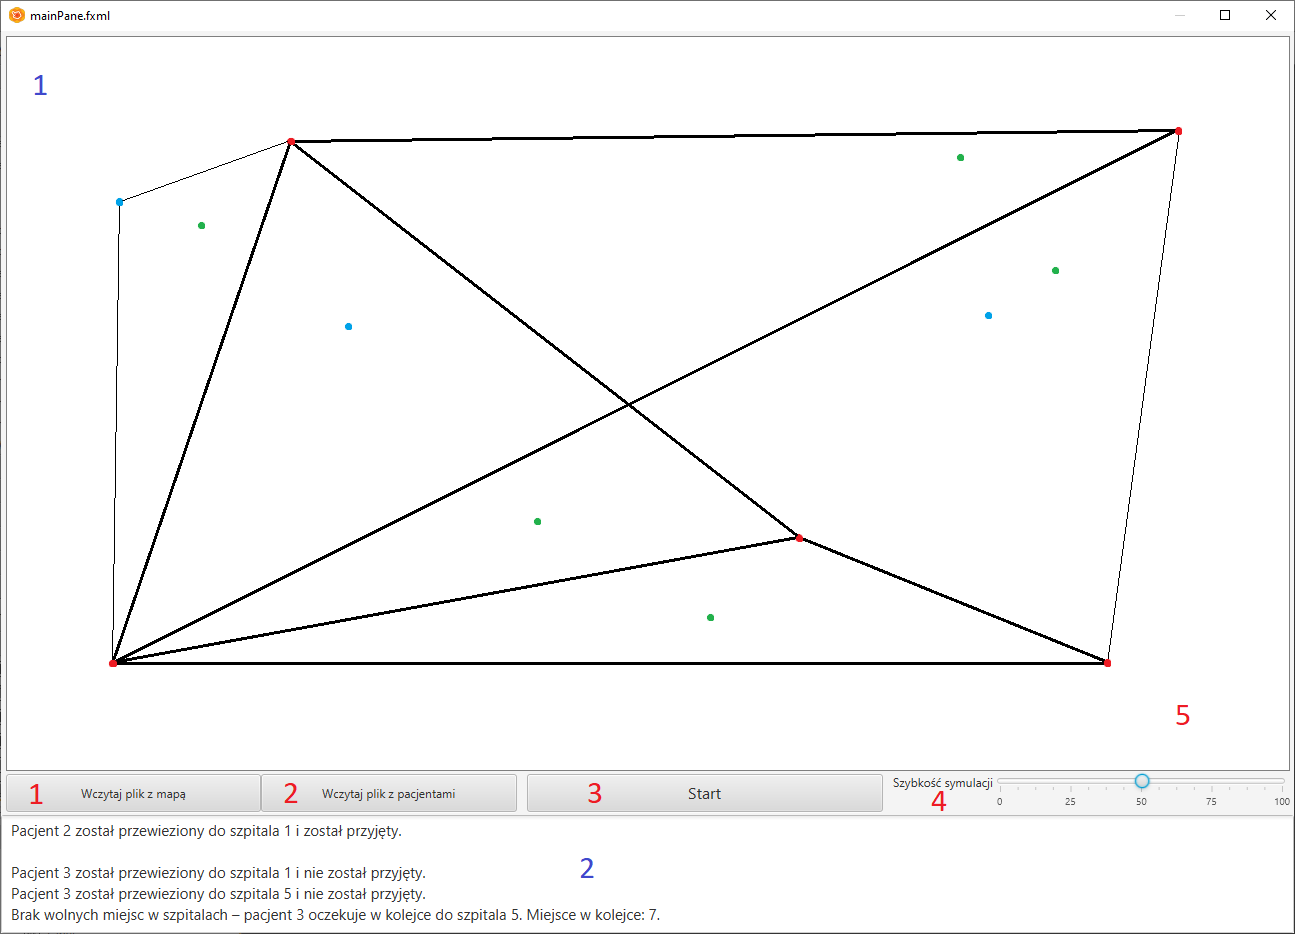
\includegraphics[scale=0.4]{GUI_impl.png}
    \end{center}
    \subsection{Elementy wyjściowe (kolor niebieski):}
    \begin{enumerate}
        \item Plansza - Wizualizuje działanie systemu, ukazując w graficzny sposób mapę.
        \item Panel wyjściowy - Pokazuje komunikaty dotyczące pacjentów.
    \end{enumerate}
    \subsection{Elementy wejściowe (kolor czerwony):}
    \begin{enumerate}
        \item Przycisk wczytania pliku z mapą - powoduje otwarcie nowego panelu z miejscem na wczytanie pliku mapy.
        \item Przycisk wczytania pliku z pacjętami - powoduje otwarcie nowego panelu z miejscem na wczytanie pliku z pacjętami.
        \item Przycisk startu - rozpoczyna symulację, po wciśnięciu zamienia się na przycisk "Stop", umożliwiając zakończenie symulacji.
        \item Suwak szybkości symulacji - dostosowuje prędkość symulacji w tym prędkość wyświetlania komunikatów.
        \item Plansza - pomimo bycia elementem wyjściowym, jest to też element wejściowy, ponieważ mamy możliwość dodawania pacjętów. Kliknięcie w dowolny obszar mapy będzie skutkowało próbą dodania pacjęta.
    \end{enumerate}
    Wszystkie elementy wejściowe będą nasłuchiwane przez słuchaczy.

\section{Testowanie}
    \subsection{Użyte narzędzia}
    Testowanie będzie odbywać się za pomocą \textbf{testów jednostkowych}, wykorzystując w tym celu technologię \textbf{JUnit 4.12}. Testy jednostkowe będą obejmowały testowanie najważniejszych metod klas modułów input i app. Poprawność działania graficznego interfejsu użytkownika będzie testowana ręcznie w trakcie powstawania programu.

    Testowanie będzie odbywać się za pomocą \textbf{testów jednostkowych}, wykorzystując w tym celu technologię \textbf{JUnit}. Testy jednostkowe będą obejmowały testowanie poszczególnych modułów, niektórych klas i ich ważniejszych funkcji. Poprawność działania graficznego interfejsu użytkownika będzie testowana ręcznie w trakcie powstawania programu.
    \subsection{Konwencja}
    \subsubsection{Nazwy testów}
    Nazwy testów jednostkowych będą pisane wykorzystując konwencję CamelCase i nazywane według następującego wzoru:
    \begin{center}
        should + [Przewidywane zachowanie] + When + [Warunek]
    \end{center}
    \subsubsection{Wnętrze funkcji testowych}
    Wewnątrz funkcji testowych zostanie zastosowana konwencja \textbf{given, when, then}. Kod każdej metody testowej zostanie podzielony na 3 części:
    \begin{itemize}
        \item given - Założenia początkowe. W tej sekcji ustawiamy stan programu zgodnie z przypadkiem, który testujemy.
        \item when - Wykonanie akcji, której poprawność działania testujemy.
        \item then - Sprawdzenie czy testowana fulknjonalność zachowała się zgodnie z oczekiwaniami, wykorzystując asercje.
    \end{itemize}
    Powyższe etykiety będą występowały w każdej funkcji testującej jako komentarz poprzedzający daną sekcję.
    \subsection{Warunki brzegowe i przypadki szczególne}
    Przetestowane zostanie działanie metod modułu input z błędnymi danymi wejściowymi oraz danymi testującymi warunki brzegowe programu. Sytuacje, które będą podlegały testowaniu:
    \begin{itemize}
        \item Bardzo duża liczba pacjentów.
        \item Współrzędne szpitali/obiektów znacznie oddalone od siebie - bardzo duża mapa do wygenerowania.
        \item Nieodpowiednia liczba znaków '|' i '\#' w pliku wejściowym.
        \item Brak szpitali/dróg/pacjentów.
        \item Nieodpowiednie wartości - niespełniające odpowiednich warunków lub uniemożliwiające konwersję (np. wartość ma być dodatnią liczbą całkowitą).
        \item Bardzo duża liczba szpitali.
        \item Niezgodność identyfikatorów - powtórzenie dwa razy tego samego identyfikatora dla tego samego typu obiektów lub nawiązanie do niestniejącego id (np. droga do szpitala, który nie istnieje).
        \item Próba dodania dwóch obiektów na tych samych współrzędnych.
        \item Próba dodania pacjenta poza granicami państwa.
    \end{itemize}

\end{document}